\documentclass[../Thesis-IJspeert.tex]{subfiles}

\begin{document}

\graphicspath{ {"Appendices/figs/"} }
\pgfplotsset{table/search path={"Appendices/data/"}}

\begin{appendices}

\chapter{Stochastic cavity loading}
\label{appendixA}
For a total number of atoms $N$ in a control volume $V$ (see \autoref{volume}), the probability $P(N,n,\alpha)$ that $n$ atoms occupy the cavity mode volume $\delta V$ is given by the binomial distribution:
\begin{equation}
\label{binomial}
P(N,n,\alpha)=\frac{N!}{\left(N-n\right)!n!}\alpha^n\left(1-\alpha\right)^{N-n}\,,
\end{equation}
where $\alpha=\sfrac{\delta V}{V}$. A quantity of interest is the following ratio $\chi$ of probabilities:
\begin{equation}
\label{successratio}
\chi=\frac{P(1,N,\alpha) P(1,N,\alpha)}{2 P(2,N,\alpha) P(0,N,\alpha)}\,,
\end{equation}
which represents the success ratio of single atom loading in each of two identical cavities versus double loading in one of two identical cavities.
\tikzstyle{int}=[draw, fill=blue!20, minimum size=2em]
\tikzstyle{init} = [pin edge={to-,thin,black}]
\begin{figure}[h]
	\centering
	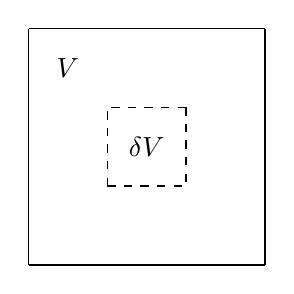
\begin{tikzpicture}
	\coordinate (O) at (0,0);
	\draw (0.5,0.5) node {$\delta V$};
	
	\draw[dashed] (0,0) -- (0,1);
	\draw[dashed] (0,0) -- (1,0);
	\draw[dashed] (1,1) -- (0,1);
	\draw[dashed] (1,1) -- (1,0);
	
	\draw (-0.5,1.5) node {$V$};
	\draw[semithick] (-1,-1) -- (2,-1);
	\draw[semithick] (2,2) -- (-1,2);
	\draw[semithick] (2,-1) -- (2,2);
	\draw[semithick] (-1,-1) -- (-1,2);
	\end{tikzpicture}
	\caption{Control volume $V$ with a cavity mode volume $\delta V$ of interest.}
	\label{volume}
\end{figure}
Using \autoref{binomial}, $\chi$ can be rewritten in terms of the total number of atoms per control volume:
\begin{equation}
\chi(N)=\frac{N}{N-1}\,.
\end{equation}
Note that in an experiment that involves stochastic cavity loading, which is the case for an atomic fountain, $N\gg1$, which implies that $\chi(N)\approx1$. This means that double loading of one cavity is as likely to occur as single atom loading in both cavities. Thus, one cannot be certain about the loading configuration in the event of a two-photon detection.

\chapter{Some Appendix}

\begin{figure}[t]
	\centering
	\begin{tikzpicture}
	\newcommand\step{0.157491}
	\newcommand\gap{0.0110096}
	
	\node[anchor=south west,inner sep=0] (image) at (0,0) {\includegraphics[width=0.85\textwidth]{{"allH"}.pdf}};
	\begin{scope}[x={(image.south east)},y={(image.north west)}]
	
	%\draw[help lines,xstep=.1,ystep=.1] (0,0) grid (1,1);
	%\foreach \x in {0,1,...,9} { \node [anchor=north] at (\x/10,0) {0.\x}; }
	%\foreach \y in {0,1,...,9} { \node [anchor=east] at (0,\y/10) {0.\y}; }
	
	\draw[thick, ->, line cap=rect] (-0.012, 1.012) -- (-0.012, -0.02) node[above left] {$n_y$};
	\draw[thick, ->, line cap=rect] (-0.012, 1.012) -- (1.02, 1.012) node[above left] {$n_x$};
	
	\draw[thick, ->, line cap=rect] (0.661, 1-0.661) -- (1.02, 1-0.661) node[above left] {$n$};
	\draw[thick, ->, line cap=rect] (0.661, 1-0.661) -- (0.661, -0.02) node[above left] {$l$};
	
	\node[align=center] at (-0.03, \step/2) {$5$};
	\node[align=center] at (-0.03, 3*\step/2 + \gap) {$4$};
	\node[align=center] at (-0.03, 5*\step/2 + 2*\gap) {$3$};
	\node[align=center] at (-0.03, 7*\step/2 + 3*\gap) {$2$};
	\node[align=center] at (-0.03, 9*\step/2 + 4*\gap) {$1$};
	\node[align=center] at (-0.03, 11*\step/2 + 5*\gap) {$0$};
	
	\node[align=center] at (\step/2, 1.035) {$0$};
	\node[align=center] at (3*\step/2 + \gap, 1.035) {$1$};
	\node[align=center] at (5*\step/2 + 2*\gap, 1.035) {$2$};
	\node[align=center] at (7*\step/2 + 3*\gap, 1.035) {$3$};
	\node[align=center] at (9*\step/2 + 4*\gap, 1.035) {$4$};
	\node[align=center] at (11*\step/2 + 5*\gap, 1.035) {$5$};
	
	\node[align=center] at (0.661-0.018, 3*\step/2 + \gap) {$0$};
	\node[align=center] at (0.661-0.018, \step/2) {$1$};
	\node[align=center] at (0.661+0.012 + \step/2, 1-0.661+0.023) {$0$};
	\node[align=center] at (0.661+0.012 + 3*\step/2 + \gap, 1-0.661+0.023) {$1$};
	
	\end{scope}
	\end{tikzpicture}
	\caption[Optical setup for generation of dipole traps and MOT.]{(Left) Optical setup for the generation of \SI{1064}{\nano\meter} dipole traps and the detection of fluorescence. A spatial light modulator (SLM) generates a tweezer array inside the glass cell, monitored via a CCD. A dichroic mirror (DM) redirects the fluorescence into a detection path, where atoms are imaged using an EMCCD camera. Numbers indicate the beam magnification factors. (Right) Optical setup for the generation of the MOT inside a glass cell using $3$ retro-reflected beams. A pair of high-NA lenses focus and image the dipole trapping light.}
	\label{cavitymodestheory} 
\end{figure}


\chapter{Some Appendix}
Let $x_{i, j}$ denote the $j$-th data point in the $i$-th group which has $n_{i}$ data points. There are $N$ such groups and thus a total of $\sum_{i=1}^{N} n_{i}=n$ data points. If the sample mean and sample variance of the $i$-th group are $m_{i}$ and $v_{i}$ respectively, then we have
\begin{equation}
n_{i} \cdot m_{i}=\sum_{j=1}^{n_{i}} x_{i, j} \quad \text { and } \quad\left(n_{i}-1\right) v_{i}=\sum_{j=1}^{n_{i}}\left(x_{i, j}-m_{i}\right)^{2}
\end{equation}
It follows that $\sum_{i=1}^{N} \sum_{j=1}^{n_{i}} x_{i, j}=\sum_{i=1}^{N} n_{i} \cdot m_{i}=n \cdot m$ where $m$ is the overall mean of the $n$ data points. Similarly, the sum $\sum_{i=1}^{N}\left(n_{i}-1\right) v_{i}=\sum_{i=1}^{N} \sum_{j=1}^{n_{i}}\left(x_{i, j}-m_{i}\right)^{2}$ can be recognized as the sum of the squared deviations of the data points from the means of their respective groups. This is not quite what we want for calculating the variance of the $n$ data points: we need to know the sum of the squared deviations from $m$. Fortunately, all that is needed is a little algebra. We have that
\begin{equation}
\begin{aligned}
	\sum_{i=1}^{N} \sum_{j=1}^{n_{i}}\left(x_{i, j}-m\right)^{2} & =\sum_{i=1}^{N}\left[\sum_{j=1}^{n_{i}}\left(x_{i, j}^{2}-2 x_{i, j} m+m^{2}\right)\right] \\
	& =\sum_{i=1}^{N}\left[\left(\sum_{j=1}^{n_{i}} x_{i, j}^{2}\right)-2 n_{i} m_{i} m+n_{i} m^{2}\right] \\
	& =\sum_{i=1}^{N}\left[\left(\sum_{j=1}^{n_{i}} x_{i, j}^{2}\right)+n_{i}\left(m^{2}-2 m_{i} m+m_{i}^{2}\right)-n_{i} m_{i}^{2}\right] \\
	& =\sum_{i=1}^{N}\left[n_{i}\left(m_{i}-m\right)^{2}+\sum_{j=1}^{n_{i}}\left(x_{i, j}^{2}-m_{i}^{2}\right)\right] \\
	& =\sum_{i=1}^{N}\left[n_{i}\left(m_{i}-m\right)^{2}+\sum_{j=1}^{n_{i}}\left(x_{i, j}^{2}-2 x_{i, j} m_{i}+m_{i}^{2}\right)\right] \\
	& =\sum_{i=1}^{N}\left[n_{i}\left(m_{i}-m\right)^{2}+\sum_{j=1}^{n_{i}}\left(x_{i, j}-m_{i}\right)^{2}\right] \\
	& =\sum_{i=1}^{N}\left[n_{i}\left(m_{i}-m\right)^{2}+\left(n_{i}-1\right) v_{i}\right] .
\end{aligned}
\end{equation}
All that remains is to divide both sides by $n-1$ and we are done.

\chapter{Some Appendix 2}
In statistics, a binomial proportion confidence interval is a confidence interval for the probability of success calculated from the outcome of a series of success–failure experiments (Bernoulli trials). In other words, a binomial proportion confidence interval is an interval estimate of a success probability p when only the number of experiments n and the number of successes nS are known.

There are several formulas for a binomial confidence interval, but all of them rely on the assumption of a binomial distribution. In general, a binomial distribution applies when an experiment is repeated a fixed number of times, each trial of the experiment has two possible outcomes (success and failure), the probability of success is the same for each trial, and the trials are statistically independent. Because the binomial distribution is a discrete probability distribution (i.e., not continuous) and difficult to calculate for large numbers of trials, a variety of approximations are used to calculate this confidence interval, all with their own tradeoffs in accuracy and computational intensity. 

The Wilson score interval is an improvement over the normal approximation interval in multiple respects. It was developed by Edwin Bidwell Wilson (1927) Unlike the symmetric normal approximation interval (above), the Wilson score interval is asymmetric. It does not suffer from problems of overshoot and zero-width intervals that afflict the normal interval, and it may be safely employed with small samples and skewed observations. The observed coverage probability is consistently closer to the nominal value, $1-\alpha$.

Like the normal interval, the interval can be computed directly from a formula.

Wilson started with the normal approximation to the binomial:
\begin{equation}
z \approx \frac{(p-\hat{p})}{\sigma_{n}}
\end{equation}
with the analytic formula for the sample standard deviation given by
\begin{equation}
\sigma_{n}=\sqrt{\frac{p(1-p)}{n}} .
\end{equation}
Combining the two, and squaring out the radical, gives an equation that is quadratic in $p$ :
\begin{equation}
(\hat{p}-p)^{2}=z^{2}  \frac{p(1-p)}{n}
\end{equation}
Transforming the relation into a standard-form quadratic equation for $p$, treating $\hat{p}$ and $n$ as known values from the sample (s the value of $z$ that corresponds to the desired confidence for the estimate of $p$ gives this:
\begin{equation}
\left(1+\frac{z^{2}}{n}\right) p^{2}+\left(-2 \hat{p}-\frac{z^{2}}{n}\right) p+\left(\hat{p}^{2}\right)=0,
\end{equation}
where all of the values in parentheses are known quantities. The solution for $p$ estimates the upper and lower limits of the cor Hence the probability of success $p$ is estimated by
\begin{equation}
p \approx\left(w^{-}, w^{+}\right)=\frac{1}{1+\frac{z^{2}}{n}}\left(\hat{p}+\frac{z^{2}}{2 n}\right) \pm \frac{z}{1+\frac{z^{2}}{n}} \sqrt{\frac{\hat{p}(1-\hat{p})}{n}+\frac{z^{2}}{4 n^{2}}}
\end{equation}
or the equivalent
\begin{equation}
p \approx \frac{n_{S}+\frac{1}{2} z^{2}}{n+z^{2}} \pm \frac{z}{n+z^{2}} \sqrt{\frac{n_{S} n_{F}}{n}+\frac{z^{2}}{4}} .
\end{equation}

The practical observation from using this interval is that it has good properties even for a small number of trials and / or an e Intuitively, the center value of this interval is the weighted average of $\hat{p}$ and $\frac{1}{2}$, with $\hat{p}$ receiving greater weight as the sample the center value corresponds to using a pseudocount of $\sfrac{1}{2} z^{2}$, the number of standard deviations of the confidence interval: count of successes and of failures to yield the estimate of the ratio. For the common two standard deviations in each direction \SI{95}{\percent} coverage, which itself is approximately 1.96 standard deviations), this yields the estimate $\left(n_{S}+2\right) /(n+4)$, which is known as the "plus four rule".


\chapter{Spherical Tensors}
\label{sphericaltensors}
Spherical tensors are described using the set of spherical basis vectors $\{\hat{e}_1, \hat{e}_0, \hat{e}_{-1}\}$ that are defined as
\begin{align}
\begin{split}
	\hat{e}_{\pm 1} &:= \frac{\mp(\hat{e}_x\pm i \hat{e}_y)}{\sqrt{2}}\\ \hat{e}_0&:=\hat{e}_z\,,
\end{split}
\end{align}
in terms of the Cartesian unit vectors. The contravariant components $A^q$ of a vector $\vec{A}$ are
\begin{align}
	A^q=\hat{e}_q^*\cdot \vec{A}\,,
\end{align}
which allow us to decompose $\vec{A}$ in the spherical basis as
\begin{align}
	\vec{A}=\sum_q A^q \hat{e}_q\,.
\end{align}
In the dual basis, which consists of the basis vectors $\hat{e}^q=\hat{e}_q^*$ such that $\hat{e}^q\hat{e}_{q'}=\delta_{qq'}$, the covariant components of $\vec{A}$ are
\begin{align}
	A_q = \hat{e}_q\cdot \vec{A}\,,
\end{align} 
such that the decomposition reads
\begin{align}
	\vec{A}=\sum_q A_q \hat{e}^q\,.
\end{align}
Note that $\hat{e}^q=\hat{e}_q^*=(-1)^q\hat{e}_{-q}$, which gives rise to various notations for the decomposition of $\vec{A}$ and the fact that $A^0=A_0$ and $A^{\pm 1}= -A_{\mp 1}$. Using different representations, the inner product of two vectors $\vec{A}$ and $\vec{B}$ in the spherical basis can be written as
\begin{align}
\begin{split}
	\vec{A}\cdot\vec{B}= A^q \hat{e}_q B_{q'} \hat{e}^{q'} = A^q B_q &= A^1 B_1 + A^0 B_0 + A^{-1} B_{-1} \\&= -A^1 B^{-1} + A^0 B^0 - A^{-1} B^1 \\&= \sum_q (-1)^q A^q B^{-q} \\&= \sum_q (-1)^q A_q B_{-q}\,.
\end{split}
\end{align}
When it comes to converting Cartesian tensor components into their spherical tensor counterparts, the approach depends on the rank of the tensor. A rank-$0$ tensor T will simply have one spherical tensor component $T_0^{(0)}=T$. For a Cartesian rank-$1$ tensor $T_\mu$, the spherical tensor components $T^{(1)}_q$ will be the covariant components $T_q$ as described above. The reason is that the covariant components rotate in the same way as the spherical harmonics, as opposed to the contravariant elements. For a rank-$2$ tensor $T_{\mu\nu}$, the trick involves writing the tensor as the direct product of two rank-$1$ tensors: $T_{\mu\nu}=A_\mu B_\nu$. The spherical tensor components $T_q^{(k)}$ can then be obtained by coupling the spherical components $A^{(1)}_{q_1}$ and $B^{(1)}_{q_2}$ like angular momenta via the Clebsch–Gordan coefficients, since the spherical tensor components were defined to transform in the same way as spherical harmonics:
\begin{align}
	T_q^{(k)}=\sum_{\substack{q_1q_2\\
			q_1+q_2=q}} T^{(k_1)}_{q_1} T^{(k_2)}_{q_2} \langle k_1\, q_1 ; k_2\, q_2 \vert k\, q \rangle\,,
\end{align}
where $\vert k_1 - k_2 \vert \le k \le k_1 + k_2$ and $\langle k_1\, q_1 ; k_2\, q_2 \vert k\, q \rangle$ represents the Clebsch–Gordan coefficient. Substituting $T^{(k_1)}_{q_1}=A^{(1)}_{q_1}$ and $T^{(k_2)}_{q_2}=B^{(1)}_{q_2}$ allows us to construct all spherical tensor components $\{T_0^{(0)}, T_{\pm q}^{(1)}, T_{\pm q}^{(2)}\}$. The rank-$0$ combination, for instance, is given by:
\begin{align}
	T_0^{(0)}=-\sum_{q=-1}^{1} \frac{(-1)^q}{\sqrt{3}}A^{(1)}_q B^{(1)}_{-q}=-\frac{\vec{A}\cdot\vec{B}}{\sqrt{3}}\,,
\end{align}
rewritten in terms of the inner product of the vectors $\vec{A}$ and $\vec{B}$. Similarly, the rank-$1$ combination can be evaluated, giving rise to the following three components:
\begin{align}
\begin{split}
T_1^{(1)} &= \frac{1}{\sqrt{2}}(A_1B_0-A_0B_1)\\
T_0^{(1)} &= \frac{1}{\sqrt{2}}(A_1B_{-1}-A_{-1}B_1)\\
T_{-1}^{(1)} &= \frac{1}{\sqrt{2}}(A_0B_{-1}-A_{-1}B_0)\,,
\end{split}
\end{align}
which can be summarised in terms of the spherical components of the cross product $\vec{A}\times\vec{B}$:
\begin{align}
	T_q^{1}=\frac{i}{\sqrt{2}}(\vec{A}\times\vec{B})_q\,.
\end{align}
Lastly, the rank-$2$ components are
\begin{align}
\begin{split}
T_{\pm 2}^{(2)} &= A_{\pm 1}B_{\pm 1}\\
T_{\pm 1}^{(2)} &= \frac{1}{\sqrt{2}}(A_{\pm 1}B_{0}+A_{0}B_{\pm 1})\\
T_{0}^{(2)} &= \frac{1}{\sqrt{6}}(A_1B_{-1}+2A_0B_0+A_{-1}B_1)\,.
\end{split}
\end{align}
All of these spherical tensor components can subsequently be written in terms of the Cartesian tensor components $T_{\mu\nu}$ by expressing all instances of $A_{q_1}$ and $B_{q_2}$ in the Cartesian basis:
\begin{align}
\label{sphericalintermsofcartesian}
\begin{split}
T_0^{(0)}&=-\frac{1}{\sqrt{3}}\left[T_{xx}+T_{yy}+T_{zz}\right]\\
T_{\pm 1}^{(1)} &=\frac{1}{2}\left[T_{zx}-T_{xz}\pm i(T_{zy}-T_{yz})\right]\\
T_0^{(1)} &=\frac{i}{\sqrt{2}}\left[T_{xy}-T_{yx}\right]\\
T_{\pm 2}^{(2)} &= \frac{1}{2}\left[T_{xx}-T_{yy}\pm i (T_{xy}+T_{yx})\right]\\
T_{\pm 1}^{(2)} &= \frac{1}{2}\left[\mp (T_{xz}+T_{zx}) - i (T_{yz}+T_{zy})\right]\\
T_{0}^{(2)} &= -\frac{1}{\sqrt{6}}\left[T_{xx}+T_{yy}-2T_{zz}\right]\,.
\end{split}
\end{align}
We note that the rank-$0$, rank-$1$ and rank-$2$ spherical components relate directly to the isotropic, antisymmetric and symmetric traceless parts of the tensor, respectively. An important result from representation theory is the Wigner-Eckart theorem, which states that, given a tensor operator $T^{(k)}$, the matrix elements of its spherical component $T^{(k)}_q$ between two angular momentum eigenstates $\vert j\, m\rangle$ and $\vert j'\, m'\rangle$ can be decomposed as
\begin{align}
\label{wignereckart}
	\langle j\, m \vert  T^{(k)}_q \vert j'\, m' \rangle = (-1)^{2k}\langle j \| T^{(k)} \| j' \rangle \langle j\, m \vert j'\, m'; k\, q \rangle\,.
\end{align}
This factorisation involves a Clebsch–Gordan coefficient $\langle j\, m \vert j'\, m'; k\, q \rangle$ that encapsulates all orientation dependence of the matrix element and the so-called reduced matrix element $\langle j \| T^{(k)} \| j' \rangle$, which does not depend on $m$, $m′$, nor $q$ and is therefore orientation independent. The inverse relation is given by
\begin{align}
\label{inversewigner}
\langle j \| T^{(k)} \| j' \rangle = (-1)^{2k}\sum_{m'q} \langle j\, m \vert  T^{(k)}_q \vert j'\, m' \rangle \langle j\, m \vert j'\, m'; k\, q \rangle\,.
\end{align}
Through the use of the Wigner-Eckart theorem, one can derive the following relation involving the conjugated reduced matrix element:
\begin{align}
\label{ccreducedmatrixelement}
	\langle j' \| T^{(k)} \| j \rangle = (-1)^{j'-j}\sqrt{\frac{2j+1}{2j'+1}}\langle j \| T^{(k)} \| j' \rangle^*\,.
\end{align}
Now assume that we have a reduced matrix element defined as $\langle j \| T^{(k)} \| j' \rangle := \langle j_1\, j_2\, j \| T^{(k)} \| j_1'\,j_2'\,j' \rangle$ between angular momentum states of $\hat{J}=\hat{J}_1+\hat{J}_2$. If $T^{(k)}$ only acts on the states that correspond to $\hat{J}_1$ (and not $\hat{J}_2$), then $\langle j \| T^{(k)} \| j' \rangle$ can be written in terms of a reduced matrix element that involves only $j_1$ and $j_1'$:
\begin{align}
\label{reducedmatrixelementonecomponent}
\begin{split}
\langle j \| T^{(k)} \| j' \rangle &= \delta_{j_2 j_2'} (-1)^{j'+j_1+k+j_2}\sqrt{(2j'+1)(2j_1+1)}\\ &\hspace{8em}\times\tj{j_1}{j_1'}{k}{j'}{j}{j_2} \langle j_1 \| T^{(k)} \| j_1' \rangle \,.
\end{split}
\end{align}
For a tensor product $T^{(k)}=U^{(k_1)}V^{(k_2)}$ where both $U^{(k_1)}$ and $V^{(k_2)}$ act on the same angular momentum space, the reduced matrix element of $T^{(k)}$ can be decomposed as follows
\begin{align}
\label{splitreducedmatrixelement}
\begin{split}
	\langle j \| T^{(k)} \| j' \rangle = (-1)^{k+j+j'}\sum_{j''}\sqrt{(2j''+1)(2k+1)} \tj{k_1}{k_2}{k}{j'}{j}{j''} \\ \times \langle j \| U^{(k_1)} \| j'' \rangle \langle j'' \| V^{(k_2)} \| j' \rangle\,.
\end{split}
\end{align}
When it comes to Wigner-6j symbols, there are a few useful relations that we will discuss next. The first is the orthogonality relation:
\begin{align}
\label{orthogonality6j}
& \sum_j(2 j+1)\left(2 j''+1\right)\tj{j_1}{j_2}{j}{j_3}{j_4}{j'}\tj{j_1}{j_2}{j}{j_3}{j_4}{j''}=\delta_{j' j''}\,.
\end{align}
The second relation is the Biedenharn–Elliott sum rule:
\begin{align}
\begin{split}
&\tj{j_1}{j_2}{j_{12}}{j_3}{j_{123}}{j_{23}}\tj{j_{23}}{j_1}{j_{123}}{j_4}{j}{j_{14}}\\ &\hspace{3em}=\sum_{j_{124}}(-1)^{j_1+j_2+j_3+j_4+j_{12}+j_{23}+j_{14}+j_{123}+j_{124}+j}\left(2 j_{124}+1\right) \\
&\hspace{3em}\times\tj{j_3}{j_2}{j_{23}}{j_{14}}{j}{j_{124}} \tj{j_2}{j_1}{j_{12}}{j_4}{j_{124}}{j_{14}} \tj{j_3}{j_{12}}{j_{123}}{j_4}{j}{j_{124}}\,,
\end{split}
\end{align}
which, for a particular choice of quantum numbers, can be written in the following alternative form:
\begin{align}
\label{elliottrule}
\begin{split}
& \sum_{F'}(-1)^{F'}\left(2 F'+1\right)\tj{1}{1}{2}{F}{F}{F'}\tj{J}{J'}{1}{F'}{F}{I}^2\\
&\hspace{3em}=(-1)^{-\left(2 J+J'+2 F+I\right)}\tj{1}{1}{2}{J}{J}{J'}\tj{J}{J}{2}{F}{F}{I}\,,
\end{split}
\end{align}
where we have used the fact that the 6-j symbol is invariant under any permutation of the columns and under the exchange of upper and lower arguments in any two columns.


\chapter{Rotating Frame Transformation}
\label{rotatingframeapp}
Transforming a Hamiltonian to the rotating frame simplifies the time dependence of the corresponding quantum states. Consider for example a Hamiltonian that can be decomposed into a time-independent part $\hat{\mathcal{H}}_0$ and a time-dependent part $\hat{\mathcal{H}}_1(t)$ as $\hat{\mathcal{H}}(t) = \hat{\mathcal{H}}_0 + \hat{\mathcal{H}}_1(t)$. The system dynamics are governed by the Schrödinger equation:
\begin{align}
\frac{\partial}{\partial t} \lvert \psi(t) \rangle &= -\frac{i}{\hbar} \hat{\mathcal{H}}(t) \lvert \psi(t) \rangle\,,
\end{align}
which has the following formal solution:
\begin{align}
\lvert \psi(t) \rangle &= \hat{U}(t, t_0) \lvert \psi(t_0) \rangle\,.
\end{align}
The unitary time evolution operator $\hat{U}(t, t_0)$ is given in terms of the following time-ordered exponential:
\begin{align}
\hat{U}(t, t_0) &= \mathcal{T} \exp { -\frac{i}{\hbar} \int_{t_0}^{t} \hat{\mathcal{H}}(\tau) \, d\tau }\,.
\end{align}
Now, instead of working with $\lvert \psi(t) \rangle$, we define a new state vector $\lvert \phi(t) \rangle$:
\begin{align}
\lvert \phi(t) \rangle &= \hat{R}(t) \lvert \psi(t) \rangle\,,
\end{align}
where $\hat{R}(t)$ represents an arbitrary (unitary) rotation operator, such that $\hat{R}^{\dagger}(t) \hat{R}(t) = \hat{R}(t) \hat{R}^{\dagger}(t) = \mathbb{I}$. Now let us find the time dependence of this newly defined state vector, which essentially is the left-hand side of the Schrödinger equation:
\begin{align}
\begin{split}
\frac{\partial}{\partial t} \lvert \phi(t) \rangle &= \frac{\partial}{\partial t} \left( \hat{R}(t) \lvert \psi(t) \rangle \right) \\
&= \left( \frac{\partial}{\partial t} \hat{R}(t) \right) \lvert \psi(t) \rangle + \hat{R}(t) \frac{\partial}{\partial t} \lvert \psi(t) \rangle \\
&= \left( \frac{\partial}{\partial t} \hat{R}(t) \right) \lvert \psi(t) \rangle - \frac{i}{\hbar} \hat{R}(t) \hat{\mathcal{H}}(t) \lvert \psi(t) \rangle \\
&= \left( \frac{\partial}{\partial t} \hat{R}(t) \right) \hat{R}^{\dagger}(t) \lvert \phi(t) \rangle - \frac{i}{\hbar} \hat{R}(t) \hat{\mathcal{H}}(t) \hat{R}^{\dagger}(t) \lvert \phi(t) \rangle \\
&= -\frac{i}{\hbar} \left( i \hbar \left( \frac{\partial}{\partial t} \hat{R}(t) \right) \hat{R}^{\dagger}(t) + \hat{R}(t) \hat{\mathcal{H}}(t) \hat{R}^{\dagger}(t) \right) \lvert \phi(t) \rangle \\
&= -\frac{i}{\hbar} \hat{\mathcal{H}}'(t) \lvert \phi(t) \rangle\,.
\end{split}
\end{align}
In the final line, we observe that our new state vector $\lvert \phi(t) \rangle$ obeys the Schrödinger equation with a modified Hamiltonian $\hat{\mathcal{H}}'(t)$. The transformed Hamiltonian in the rotating frame is thus given by
\begin{align}
\hat{\mathcal{H}}'(t) = i \hbar \left( \frac{\partial}{\partial t} \hat{R}(t) \right) \hat{R}^{\dagger}(t) + \hat{R}(t) \hat{\mathcal{H}}(t) \hat{R}^{\dagger}(t)\,.
\end{align}
A particularly useful choice for the rotation operator is $\hat{R}(t) = \hat{U}_0^\dagger(t, t_0)$, where $\hat{U}_0(t, t_0)$ denotes the unitary evolution operator for the time-independent part of $\hat{\mathcal{H}}(t)$:
\begin{align}
\hat{U}_0(t, t_0) = \exp{-\frac{i}{\hbar} (t - t_0) \hat{\mathcal{H}}_0}\,.
\end{align}
In this case, the transformed Hamiltonian acquires the following form:
\begin{align}
\hat{\mathcal{H}}'(t) = \hat{U}_0^{\dagger}(t, t_0) \hat{\mathcal{H}}_1(t) \hat{U}_0(t, t_0)\,,
\end{align}
which is also referred to as the Hamiltonian in the interaction picture.
\end{appendices}

\end{document}
